\documentclass[12pt]{article}
\everymath{\displaystyle}
\usepackage{unicode-math}
\usepackage{pgfplots}
\pgfplotsset{compat=1.18}
\usepackage{amsmath}


\usepackage[margin=1in]{geometry}
\usepackage{tcolorbox}
\usepackage{graphicx}
\usepackage{tikz}
\usepackage{amssymb}
\usepackage{enumitem}
\usepackage{titlesec}
\usepackage{fancyhdr}
\usepackage{pifont}
\usepackage{xcolor}
\newcounter{questionnum}
\setcounter{questionnum}{0}
\usepackage{eso-pic} % for page background

% --------- 主题颜色设置 ---------
\definecolor{novelblue}{RGB}{70,60,150}
\definecolor{headerbg}{RGB}{240,240,255}

\pagestyle{fancy}
\fancyhf{}
\renewcommand{\headrulewidth}{0.4pt}
\renewcommand{\headrule}{\hbox to\headwidth{\color{novelblue}\leaders\hrule height 0.4pt\hfill}}

% --------- 页眉背景色条 ---------
\newcommand{\headbackground}{
  \AddToShipoutPictureBG*{
    \begin{tikzpicture}[remember picture, overlay]
      \fill[blue!5!purple!10] (current page.north west) rectangle ([yshift=-60pt]current page.north east);
    \end{tikzpicture}
  }
}

% --------- 页眉设置 ---------
\pagestyle{fancy}
\fancyhf{}
\renewcommand{\headrulewidth}{0pt}
\fancyhead[L]{\color{novelblue}\textbf{\textbf{Novel Prep} }}
\fancyhead[C]{\color{novelblue}\textbf {SAT Preparation}}
\fancyhead[R]{\color{novelblue}\textbf{Jack Zeng}}


\newtcolorbox{SATCard}[1][]{%
  enhanced,
  colback=white,
  colframe=novelblue,
  coltitle=white,
  boxrule=0.6pt,
  arc=4pt,
  boxsep=5pt,
  left=8pt, right=8pt, top=10pt, bottom=10pt,
  sharp corners=south,
  drop shadow south east,
  #1
}

% --------- 顶部 Mark for Review 栏 ---------
\newcommand{\markforreview}{
  \stepcounter{questionnum} % 自动递增题号
  \begin{tikzpicture}[scale=1.1]
    % 黑色题号
    \fill[black] (0,0) rectangle (0.8,0.6);
    \node[white, font=\bfseries\large] at (0.4,0.3) {\thequestionnum};

    % 灰底主栏
    \fill[gray!10] (0.8,0) rectangle (14.5,0.6);

    % Mark for Review
    \node[anchor=west, font=\small] at (1.2,0.3) {\ding{72} \hspace{2pt}Mark for Review};

    % ABC 按钮区域
    \draw[thick, rounded corners=3pt] (13.5,0.12) rectangle (14.5,0.48);
    \node[font=\bfseries\normalsize] at (14.0,0.3) {ABC};
  \end{tikzpicture}


  \newcommand{\choiceboxcircled}[2]{%
  \begin{tcolorbox}[
    colback=white,
    colframe=black,
    boxrule=0.5pt,
    rounded corners=6pt,
    left=6pt, right=6pt, top=6pt, bottom=6pt,
    width=\linewidth
  ]
    \textbf{\large\textcircled{\textbf{#1}}} \ #2
  \end{tcolorbox}
}
}

% --------- 选项框样式 ---------
\newcommand{\choicebox}[2]{%
  \begin{tcolorbox}[
    colback=white, 
    colframe=novelblue,
    boxrule=0.5pt, 
    rounded corners=4pt, 
    left=6pt, right=6pt, top=6pt, bottom=6pt,
    width=\linewidth
  ]
  \textbf{#1.} \ #2
  \end{tcolorbox}
}


\begin{document}
\section*{SAT Math Test II}
\noindent\markforreview
\vspace{1em}

A research manager selected 2 random samples of ovens of a certain type to estimate the average amount of time this type of oven takes to preheat to \(325^\circ F\).  
The research manager recorded the amount of time, in minutes, each oven takes to preheat to \(325^\circ F\).

Based on the first sample, the manager estimated an average of 14.2 minutes, with a margin of error of 1 minute.  
Based on the second sample, the estimate was 14.4 minutes, with a margin of error of 2.3 minutes.

Assuming the margins of error were calculated the same way, which of the following best explains why the first sample had a smaller margin of error?

\vspace{0.75em}

\choicebox{A}{The first sample contained fewer ovens than the second sample.}  
\choicebox{B}{The first sample contained more ovens than the second sample.}  
\choicebox{C}{The first sample took less time on average to preheat.}  
\choicebox{D}{The first sample took more time on average to preheat.}

\vspace{2em}
\newpage
\noindent\markforreview
\vspace{1em}

\begin{center}
    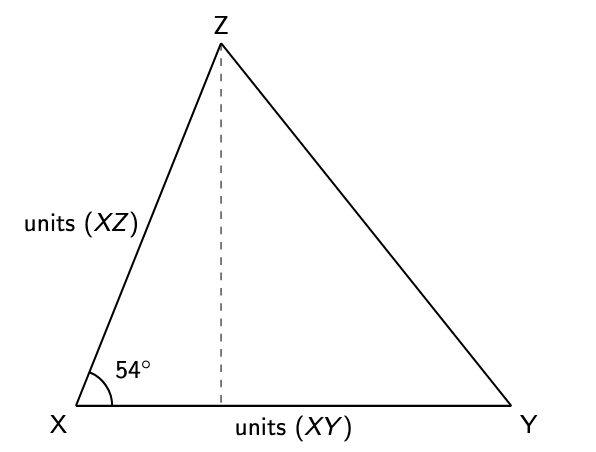
\includegraphics[width=0.45\linewidth]{f9.png}
\end{center}

In triangle \(XYZ\), \(\angle X = 54^\circ\), \(XY = 26\) units, \(XZ = 19\) units.  
What is the area, in square units, of triangle \(XYZ\)?

\vspace{0.75em}

\choicebox{A}{247}  
\choicebox{B}{494}  
\choicebox{C}{247\sin 54^\circ}  
\choicebox{D}{494\sin 54^\circ}

\vspace{2em}



\noindent\markforreview
\vspace{1em}

A circle with center \(O\) has radius 10.  
Point \(A\) lies on the circle, and chord \(AB\) subtends an angle of \(120^\circ\) at the center.  
A point \(P\) lies on the arc \(AB\), and \(PA\) is extended to meet the tangent to the circle at \(B\) at point \(T\).  
If \(BT = x\), find the exact value of \(x\).

\vspace{0.75em}

\choicebox{A}{\(10\sqrt{3}\)}  
\choicebox{B}{15}  
\choicebox{C}{10}  
\choicebox{D}{20}



\vspace{2em}
\noindent\markforreview
\vspace{1em}

In the figure, \(\triangle ABC\) is inscribed in a semicircle with diameter \(AC = 10\).  
Point \(B\) lies on the semicircle. If \(AB = 6\) and \(BC = x\), find \(x\).  
Give your answer in simplest radical form.

\vspace{0.75em}

\choicebox{A}{\(\sqrt{36}\)}  
\choicebox{B}{8}  
\choicebox{C}{\(\sqrt{44}\)}  
\choicebox{D}{\(\sqrt{64}\)}

\vspace{2em}

\noindent\markforreview
\vspace{1em}

A parabola is given by  
\[
y = x^2 - 4x + 5,
\]
and a circle by  
\[
x^2 + y^2 = 25.
\]

The parabola and circle intersect at points \(P\) and \(Q\).  
Find the distance between \(P\) and \(Q\).



\newpage
\noindent\markforreview
\vspace{1em}

Solve the equation:  
\[
\sqrt{6r} = \sqrt{r^2 - 16}
\]

What is the product of all solutions to the above equation?

\vspace{0.75em}

\choicebox{A}{4}  
\choicebox{B}{6}  
\choicebox{C}{8}  
\choicebox{D}{12}


\noindent\markforreview
\vspace{1em}

The incomplete table below summarizes the number of left-handed and right-handed students by gender for eighth-grade students at Keisel Middle School.

\begin{center}
\begin{tabular}{|c|c|c|}
\hline
\textbf{Gender} & \textbf{Left} & \textbf{Right} \\
\hline
Female &  &  \\
\hline
Male &  &  \\
\hline
Total & 18 & 122 \\
\hline
\end{tabular}
\end{center}

There are \textbf{5 times} as many right-handed female students as left-handed female students, and \textbf{9 times} as many right-handed male students as left-handed male students.

If there are a total of 18 left-handed and 122 right-handed students, which of the following is closest to the probability that a randomly selected right-handed student is female?

\vspace{0.75em}
\choicebox{A}{0.410}
\choicebox{B}{0.357}
\choicebox{C}{0.333}
\choicebox{D}{0.250}

\vspace{2em}
\newpage
\noindent\markforreview
\vspace{1em}

If shoppers enter a store at an average rate of \(r\) shoppers per minute and each stays in the store for an average time of \(T\) minutes, then the average number of shoppers in the store, \(N\), is given by the formula:

\[
N = rT
\]

The owner of the Good Deals Store estimates that 3 shoppers per minute enter the store, and each stays for 15 minutes. The store owner estimates 45 shoppers in the store at a time.

Now, for a new store, the estimate is 90 shoppers per hour, each staying 12 minutes. What percent less is this new store’s average than the original?

(Note: Ignore the percent symbol in your answer.)

\vspace{0.75em}
\choicebox{A}{57}
\choicebox{B}{58}
\choicebox{C}{59}
\choicebox{D}{60}

\vspace{2em}
\newpage
\noindent\markforreview
\vspace{1em}
A trivia tournament organizer wanted to study the relationship between the number of points a team scores in a trivia round and the number of hours that a team practices each week.

For the study, the organizer selected \textbf{55} teams at random from all trivia teams in a certain tournament. The table displays the information for the \textbf{40} teams in the sample that practiced for at least \textbf{3 hours per week.}

\begin{center}
\begin{tabular}{|c|c|c|c|}
\hline
\textbf{Hours practiced} & \textbf{6 to 13 points} & \textbf{14 or more points} & \textbf{Total} \\
\hline
\textbf{3 to 5 hours} & 6 & 4 & 10 \\
\textbf{More than 5 hours} & 4 & 26 & 30 \\
\hline
\textbf{Total} & 10 & 30 & 40 \\
\hline
\end{tabular}
\end{center}

Which of the following is the \textbf{largest population} to which the results of the study can be generalized?

\vspace{0.75em}
\choicebox{A}{All trivia teams in the tournament that scored 14 or more points.}
\choicebox{B}{The 55 trivia teams in the sample.}
\choicebox{C}{The 40 trivia teams in the sample that practiced 3+ hours/week.}
\choicebox{D}{All trivia teams in the tournament.}

\vspace{2em}

\noindent\markforreview
\vspace{1em}

A circle is centered at \((-1,1)\). Line \(t\) is tangent to the circle at point \((4,-3)\).

Which of the following points lies on line \(t\)?

\vspace{0.75em}
\choicebox{A}{\((0,\frac{5}{4})\)}
\choicebox{B}{(3,6)}
\choicebox{C}{(8,2)}
\choicebox{D}{(9,1)}

\vspace{2em}

\noindent\markforreview
\vspace{1em}

Two identical rectangular prisms have a height of \(90\ \text{cm}\), square bases, and surface area \(K\ \text{cm}^2\). Glued along a square base, the resulting surface area is \(\frac{92}{47}K\ \text{cm}^2\).

What is the side length \(s\) of the square base?

\vspace{0.75em}


\vspace{2em}

\noindent\markforreview
\vspace{1em}

In triangle \(RST\), angle \(T\) is a right angle. \(L\) lies on \(\overline{RS}\), \(K\) lies on \(\overline{ST}\), and \(LK \parallel RT\).

\textbf{Given:}
\begin{itemize}
\item \(RT = 72\ \text{units}\)
\item \(LK = 24\ \text{units}\)
\item \(\text{Area of } \triangle RST = 792\ \text{square units}\)
\end{itemize}

Find the length of \(KT\) in units.

\vspace{2em}

\noindent\markforreview
\vspace{1em}

The equation of a circle is:
\[
(x - 6)^2 + (y + 5)^2 = 16
\]
and point \(P(10, -5)\) lies on the circle. If \(PQ\) is the diameter, what are the coordinates of point \(Q\)?

\newpage
\noindent\markforreview
\vspace{1em}

The given expression can be rewritten as \(\frac{a}{4}x^2 + \frac{b}{4}x + \frac{c}{4}\), where \(a, b,\) and \(c\) are constants. What is the value of \(a + b + c\)?  
Given the expression  
\[
-16(5x - 3)^2 + 4(5x - 2)^2
\]

\vspace{0.75em}

\choicebox{A}{-112}
\choicebox{B}{-56}
\choicebox{C}{-28}
\choicebox{D}{-7}

\vspace{2em}

\noindent\markforreview
\vspace{1em}

In the given function, \(b\) is a positive constant. For every increase in the value of \(x\) by 1, the value of \(f(x)\) increases by \(c\%\), where \(0 < c < 100\).  
Which expression gives the value of \(c\) in terms of \(b\)?

\[
f(x) = 66(b)^x
\]

\vspace{0.75em}

\choicebox{A}{1 + $\frac{b}{100}$}
\choicebox{B}{b + 100}
\choicebox{C}{100(b + 1)}
\choicebox{D}{100(b - 1)}

\vspace{2em}
\newpage
\noindent\markforreview
\vspace{1em}

If \(\sin(x^\circ) = a\), which of the following must be true for all values of \(x\)?

\vspace{0.75em}

\choicebox{A}{\cos(x^\circ) = a}
\choicebox{B}{\sin(90^\circ - x^\circ) = a}
\choicebox{C}{\sin(x^2)^\circ = a^2}
\choicebox{D}{\cos(90^\circ - x^\circ) = a}

\vspace{2em}

\noindent\markforreview
\vspace{1em}

The function \(g\) is a quadratic function in the \(xy\)-plane. The graph of \(y = g(x)\) has a vertex at \((-1, -4)\) and passes through the points \((-2, -43)\) and \((1, -160)\).  
What is the value of \(g(0) - g(2)\)?

\vspace{0.75em}

\choicebox{A}{312}
\choicebox{B}{355}
\choicebox{C}{-117}
\choicebox{D}{-203}

\vspace{2em}
\newpage
\noindent\markforreview
\vspace{1em}

The mass of object A is 324\% of the mass of object B and the mass of object A is 7.2\% of the mass of object C.  
If the mass of object C is \(p\%\) of the mass of object B, what is the value of \(p\%\)?

\vspace{0.75em}

\choicebox{A}{4.5\%}
\choicebox{B}{4.5}
\choicebox{C}{45}
\choicebox{D}{450}

\vspace{2em}

\noindent\markforreview
\vspace{1em}

In the given equation, \(c\) is a constant. If the equation has exactly one solution, what is the value of \(c\)?

\[
\frac{1}{cx} = \frac{x}{76} + \frac{1}{c}
\]

\vspace{0.75em}


\newpage

\noindent\markforreview
\vspace{1em}

A parallel electric circuit contains four resistors with resistances of $p$ ohms, $q$ ohms, $s$ ohms, and 13 ohms.  
The given equation relates the resistance $R$, in ohms, of the circuit, to the resistances of the four individual resistors it contains.  
Which equation correctly expresses $R$ in terms of $p$, $q$, and $s$?

\[
\frac{1}{R} = \frac{1}{p} + \frac{1}{q} + \frac{1}{s} + \frac{1}{13}
\]

\vspace{0.75em}

\choicebox{A}{$R = \frac{13pqs}{p+q+s+13}$}
\choicebox{B}{$R = \frac{13pqs}{13qs + 13ps + 13pq + pqs}$}
\choicebox{C}{$R = \frac{13qs + 13ps + 13pq + pqs}{13pqs}$}
\choicebox{D}{$R = p + q + s + 13$}

\vspace{2em}

\noindent\markforreview
\vspace{1em}

In the given equation, $b$ is an integer. The equation has no real solutions.  
What is the least possible value of $b$?

\[
-x^2 + bx - 169 = 0
\]

\vspace{0.75em}

\choicebox{A}{26}
\choicebox{B}{25}
\choicebox{C}{-26}
\choicebox{D}{-25}

\vspace{2em}

\noindent\markforreview
\vspace{1em}

The exponential function $f$ is defined by $f(x) = ab^x$, where $a$ and $b$ are positive constants.  
If $f(n-1) = f(n) + \frac{82}{100}f(n-1)$, where $n$ is a constant, what is the value of $b$?

\vspace{0.75em}

\choicebox{A}{1}
\choicebox{B}{0.82}
\choicebox{C}{0.18}
\choicebox{D}{10}

\newpage

\section*{Additional Problems}

\noindent\markforreview
\vspace{1em}

A rectangle is inscribed in a circle such that the length of the diagonal of the rectangle is twice the length of its shortest side.  
The circumference of the circle is $114\pi$ units. What is the area, in square units, of the rectangle?

\vspace{0.75em}

\choicebox{A}{$57\sqrt{2}$}
\choicebox{B}{$57\sqrt{3}$}
\choicebox{C}{$3,\!249\sqrt{2}$}
\choicebox{D}{$3,\!249\sqrt{3}$}

\vspace{2em}
\newpage
\noindent\markforreview
\vspace{1em}

In triangle $PQR$, the measure of angle $P$ is $(3x + 5)^\circ$, the measure of angle $Q$ is $(2x + 9)^\circ$, and the measure of angle $R$ is $(4y + 5)^\circ$.  
If side $QR$ is extended through point $R$ to point $S$, and the measure of angle $PRS$ is $(x + y)^\circ$, what is the value of $x + y$?

\vspace{0.75em}

\choicebox{A}{39}
\choicebox{B}{29}
\choicebox{C}{141}
\choicebox{D}{146}

\vspace{2em}

\noindent\markforreview
\vspace{1em}

The manager of a gym selected a sample of 139 members at random to estimate the percentage of the gym’s members that would continue to pay for a membership if the price increased.  
From the survey, the manager estimates that 82\% of the gym’s members would continue to pay for a membership if the price increased, with an associated margin of error of 6.39\%.  
If the survey is repeated with a random sample of 278 members and the results are calculated in the same way, which of the following will be the most likely effect of using the larger random sample compared to the smaller random sample?

\vspace{0.75em}

\choicebox{A}{The margin of error will be lower.}
\choicebox{B}{The margin of error will be higher.}
\choicebox{C}{The estimate of the percentage of the gym’s members that would continue to pay for a membership if the price increased will be lower.}
\choicebox{D}{The estimate of the percentage of the gym’s members that would continue to pay for a membership if the price increased will be higher.}

\vspace{2em}
\newpage
\noindent\markforreview
\vspace{1em}

Given the expression $\sqrt[5]{119n \left(\sqrt[6]{119n}\right)^2}$,  
for what value of $x$ is the expression equivalent to $(119n)^{30x}$, where $n > 1$?

\vspace{0.75em}

\choicebox{A}{225}
\choicebox{B}{$\frac{8}{225}$}
\choicebox{C}{$\frac{4}{225}$}
\choicebox{D}{$\frac{2}{225}$}

\vspace{2em}

\noindent\markforreview
\vspace{1em}

The mass of object A is 483\% of the mass of object B, and the mass of object A is 0.069\% of the mass of object C.  
If the mass of object C is $p\%$ of the mass of object B, what is the value of $\frac{p}{1,\!000}$?

\vspace{0.75em}

\choicebox{A}{0.7\%}
\choicebox{B}{70}
\choicebox{C}{70\%}
\choicebox{D}{700}

\vspace{2em}
\newpage
\noindent\markforreview
\vspace{1em}

For triangle $PQR$ and triangle $STU$, angles $P$ and $S$ each measure $30^\circ$, $QR = 16$ and $TU = 12$.  
Which additional piece(s) of information is(are) sufficient to prove that triangle $PQR$ is similar to triangle $STU$?

\begin{itemize}
    \item[I] Q = $40^\circ$ and U =$110^\circ$ 
    \item[II] $\frac{PR}{SU} = \frac{4}{3}$
\end{itemize}
\vspace{0.75em}

\choicebox{A}{I is sufficient, but II is not.}
\choicebox{B}{II is sufficient, but I is not.}
\choicebox{C}{I is sufficient, and II is sufficient.}
\choicebox{D}{Neither I nor II is sufficient.}











\end{document}